% Copyright 2004 by Till Tantau <tantau@users.sourceforge.net>.
%
% In principle, this file can be redistributed and/or modified under
% the terms of the GNU Public License, version 2.
%
% However, this file is supposed to be a template to be modified
% for your own needs. For this reason, if you use this file as a
% template and not specifically distribute it as part of a another
% package/program, I grant the extra permission to freely copy and
% modify this file as you see fit and even to delete this copyright
% notice. 

%\documentclass[notes]{beamer}
\documentclass{beamer}
% There are many different themes available for Beamer. A comprehensive
% list with examples is given here:
% http://deic.uab.es/~iblanes/beamer_gallery/index_by_theme.html
% You can uncomment the themes below if you would like to use a different

%\usetheme{AnnArbor}
%\usetheme{Antibes}
%\usetheme{Bergen}
%\usetheme{Berkeley}
%\usetheme{Berlin}
%\usetheme{Boadilla}
%\usetheme{boxes}
%\usetheme{CambridgeUS}
%\usetheme{Copenhagen}
%\usetheme{Darmstadt}
%\usetheme{default}
%\usetheme{Frankfurt}
%\usetheme{Goettingen}
%\usetheme{Hannover}
%\usetheme{Ilmenau}
%\usetheme{JuanLesPins}
%\usetheme{Luebeck}
%\usetheme{Madrid}
%\usetheme{Malmoe}
%\usetheme{Marburg}
%\usetheme{Montpellier}
%\usetheme{PaloAlto}
%\usetheme{Pittsburgh}
%\usetheme{Rochester}
%\usetheme{Singapore}
%\usetheme{Szeged}
%\usetheme{Warsaw}
%\usetheme[]{metropolis}

\title{A dynamical geography of the Gulf of Mexico}

% A subtitle is optional and this may be deleted
%\subtitle{Optional Subtitle}

\author{Philippe Miron\inst{1},  Francisco J. Beron-Vera\inst{1}, Mar\'ia J. Olascoaga\inst{2}, Paula P\'erez-Brunius\inst{3}, Julio Sheinbaum\inst{3} and Gary Froyland\inst{4}}

\institute % (optional, but mostly needed)
{
  \inst{1}%
  RSMAS/ATM University of Miami, Miami, USA
  \and
  \inst{2}%
  RSMAS/OCE University of Miami, Miami, USA
  \and
  \inst{3}%
  CICESE, Ensenada, Mexico
  \and
  \inst{4}%
  University of New South Wales, Sydney, Australia
  }
% - Use the \inst command only if there are several affiliations.
% - Keep it simple, no one is interested in your street address.

\date{BIRS on Thursday, January 19}
%\date{2017 Oil Spill and Ecosystem Science Conference}
% - Either use conference name or its abbreviation.
% - Not really informative to the audience, more for people (including
%   yourself) who are reading the slides online

\subject{Applied oceanography}
% This is only inserted into the PDF information catalog. Can be left
% out. 

% If you have a file called "university-logo-filename.xxx", where xxx
% is a graphic format that can be processed by latex or pdflatex,
% resp., then you can add a logo as follows:
%\pgfdeclareimage[height=1.5cm]{logo}{GoMRi.png}
%\logo{\pgfuseimage{logo}}

% Delete this, if you do not want the table of contents to pop up at
% the beginning of each subsection:
%\AtBeginSubsection[]
%{
%  \begin{frame}<beamer>{Outline}
%  \tableofcontents[currentsection,currentsubsection]
%  \end{frame}
%}

% graphic
\graphicspath{{"2017. dynamical geography (birs)/figures/"}}
%\graphicspath{{"figures/"}}

% titlepage logo
\titlegraphic{
\begin{tikzpicture}[overlay, remember picture]
\node[at=(current page.south west), anchor=south west] {%
 
\includegraphics[width=.35\textwidth]{carthe.png} 
};
\node[at=(current page.south east), anchor=south east] {
 
\includegraphics[width=.3\textwidth]{GoMRi.png} 
};
\end{tikzpicture}
}

% bibliography
\usepackage[style=authoryear, natbib=true]{biblatex}
\addbibresource{oce.bib}
% remove annoying biblatex bug/warning
\usepackage{silence}
\WarningFilter{biblatex}{Patching footnotes failed}

% some definitions
\usepackage[utf8]{inputenc}
\usepackage[english]{babel}
\usepackage{amssymb}
\usepackage{amsfonts}
\usepackage{amsmath}
\usepackage{bbold}
\usepackage{ragged2e} % justify text in all frame
\apptocmd{\frame}{}{\justifying}{}
\usepackage{etoolbox}
\usepackage{tikz}
\usepackage{subfig}
\usepackage{multicol}
\usepackage{siunitx}
\usepackage{csquotes}
\usepackage{hyperref}
\usepackage{tikz,pgfplots}
\pgfplotsset{compat=1.12}

% Definitions.
\def\vol{\mathop{\rm area}}

\newcommand{\PF}{\mathcal{P}}
\newcommand{\ia}{\textit{a}}
\newcommand{\ib}{\textit{b}}
\newcommand{\ic}{\textit{c}}
\newcommand{\id}{\textit{d}}
\newcommand{\ie}{\textit{e}}
\newcommand{\gom}{GoM}
\let\vaccent=\v 
\renewcommand{\v}[1]{\ensuremath{\mathbf{#1}}} 
\newcommand{\minus}{\scalebox{0.5}[1.0]{$-$}}

% Let's get started
\begin{document}

\frame[plain,noframenumbering]{
\titlepage

}

\note[itemize]{
\item Present myself
\item I would lie to take a moment to thank the organizers for inviting me and letting me present the project I've been working on for the last 3 months.
\item It's a joint research with my advisors at UMiami, two colleagues in Mexico and Gary who helps us getting started using the Transfer operator.
}

\iffalse
\begin{frame}{Outline}
  \tableofcontents
  % You might wish to add the option [pausesections]
\end{frame}
\fi

\frame{\frametitle{Objectives}

Using \textbf{only} drifters data (trajectories) in the Gulf of Mexico (\gom):
\begin{itemize}
    \item Subdivide the \gom\ into regions with similar dynamics
    \item Identify sink and source (attractor and basins of attraction)
    \item Predict transport of passive and possibly non-passive tracers
\end{itemize}
}

\note[itemize]{
    \item Basically the goal of this research was to try to extract information only from drifters trajectories.
    \item We want to subdivide the \gom into closed regions with similar dynamics.
    \item and eventually be able to predict the transport of passive tracers (like oil or plastic) and possibly non-passive tracers like marine organisms.
}

% Section and subsections will appear in the presentation overview
% and table of contents.
\section{Introduction}

\frame{\frametitle{Drifters database in the \gom\ (1994-2016)}

\textbf{Problematics: non uniform data (data per year, type of drifters, time resolution)}
 
\begin{itemize}
    \item Left: initial positions
    \item Right: all trajectories data points
\end{itemize}
\begin{figure}[!ht]
  \centering
  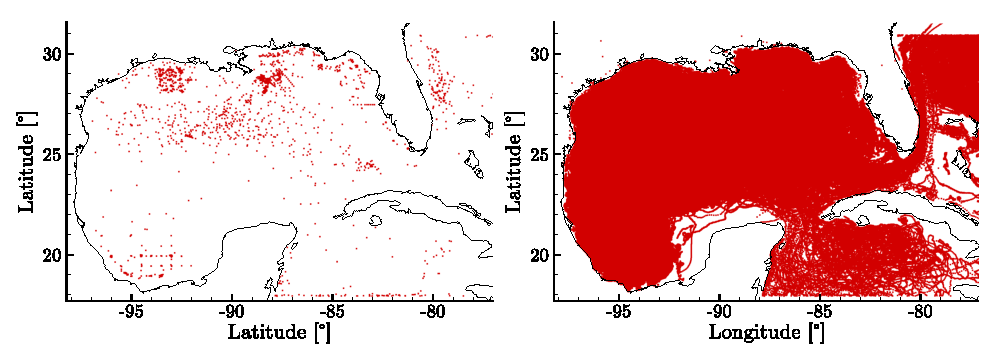
\includegraphics[width=\textwidth]{fig03}
  \label{fig:gom_bins}
\end{figure}

3312 drifters from different sources (LASER \& GLAD / CARTHE, GDP / NOAA, BOEM / SCULP, PEMEX / CICESE)
}

\note[itemize]{
    \item So first let's talk about the drifters database inside the \gom. The main characteristic of the data is that it is highly non uniform.
    \item First of all, we have drifters data in the Gulf since 1994, but it's not evenly distributed across the 22 years.
    \item There is different drifters type and their temporal resolution varies from 1 day to 15min.
    \item Left image, we see that the initial position of the drifters is concentrated on the north part of the Gulf where of the deployment occur.
    \item Has a first step, we will use all of the available data together and we will try to extract the average dynamics of the Gulf of Mexico.
}

\frame{\frametitle{Biodegradable drifters \parencite[][University of Miami]{Novelli-etal-17}}

\begin{itemize}
    \item 1000 drifters deployed during the LAgrangian Submesoscale  ExpeRiment (LASER) in 2016
    \item Total height of \SI{0.6}{m}
    \item GPS precision $\pm\SI{10}{m}$
    \item Quarter-hourly acquisition ($\sim3$ months)
\end{itemize}
\begin{figure}[!ht]
  \centering
  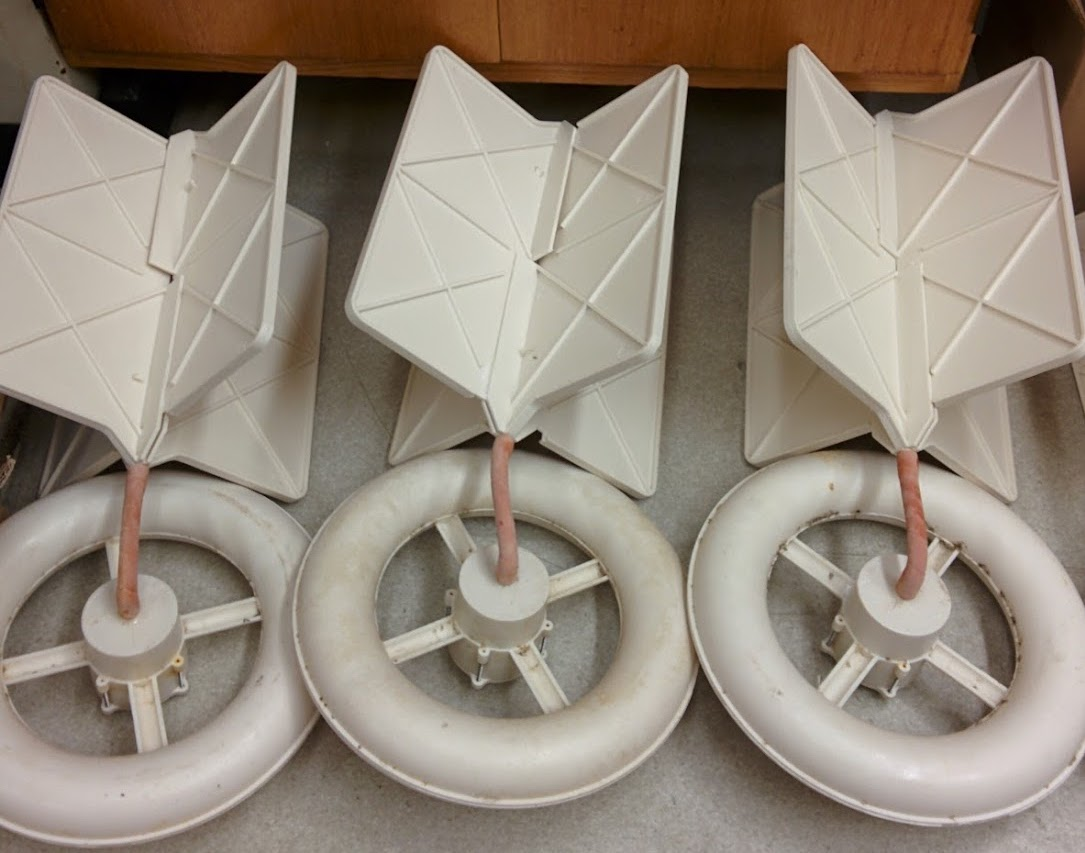
\includegraphics[angle=180,width=0.5\textwidth]{Drifters}
\end{figure}
}

\note[itemize]{
    \item These are the drifters design and use during the last experiments at the University of Miami.
    \item 1000 release last year during Laser, which is around 30\% of all the drifters database.
}

\section[Transfer Operator theory]{Theory}

\frame{\frametitle{Approximation of an attractor \parencite{Dellnitz-etal-97}}

\begin{equation*}
    \text{\underline{H\'{e}non Map}: } (x_1, x_2) \to \left(1- 1.4 x_1^2 + 0.3x_1x_2\right)
\end{equation*}

\vspace{-0.5cm}
\center{10000 iterations}
\vspace{-0.25cm}

\begin{figure}[!ht]
  \centering
  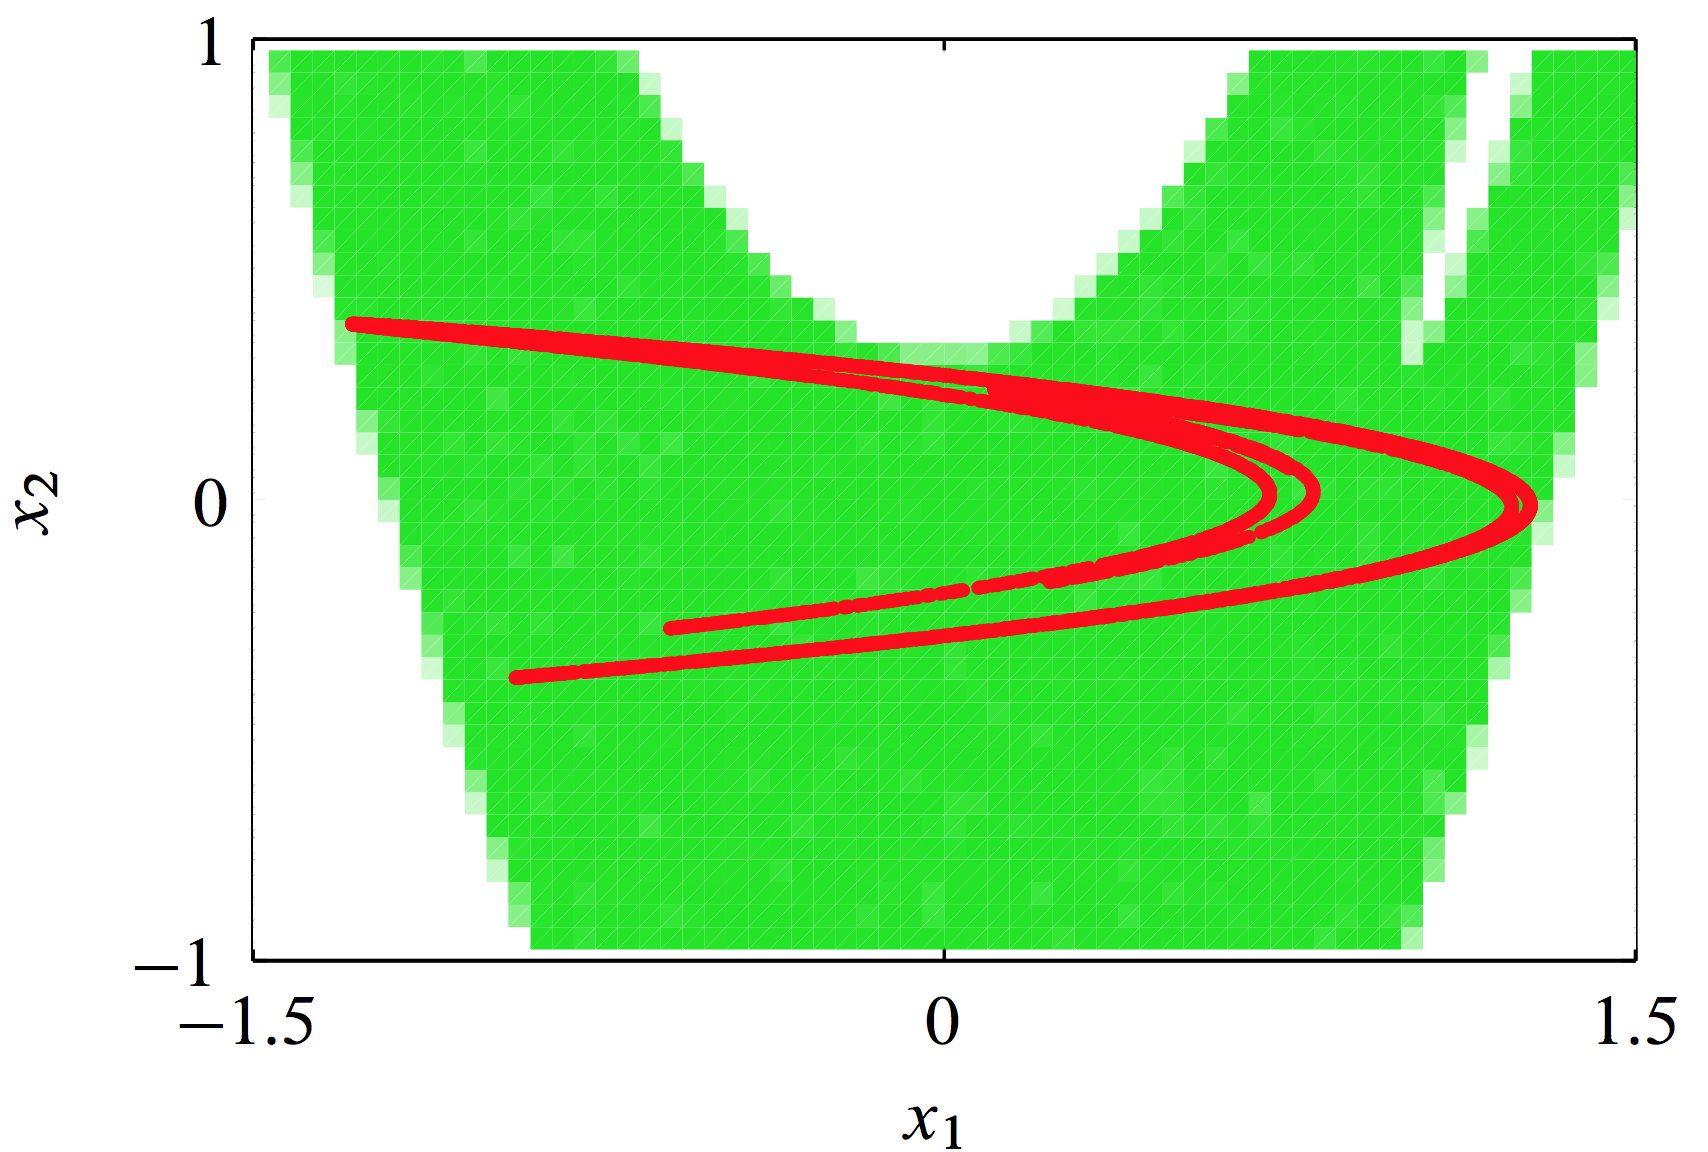
\includegraphics[width=0.35\textwidth]{henon-solution.png}
\end{figure}

\vspace{-0.7cm}
\center{1 iteration}
\vspace{-0.6cm}
\begin{figure}
    \centering
    \subfloat{{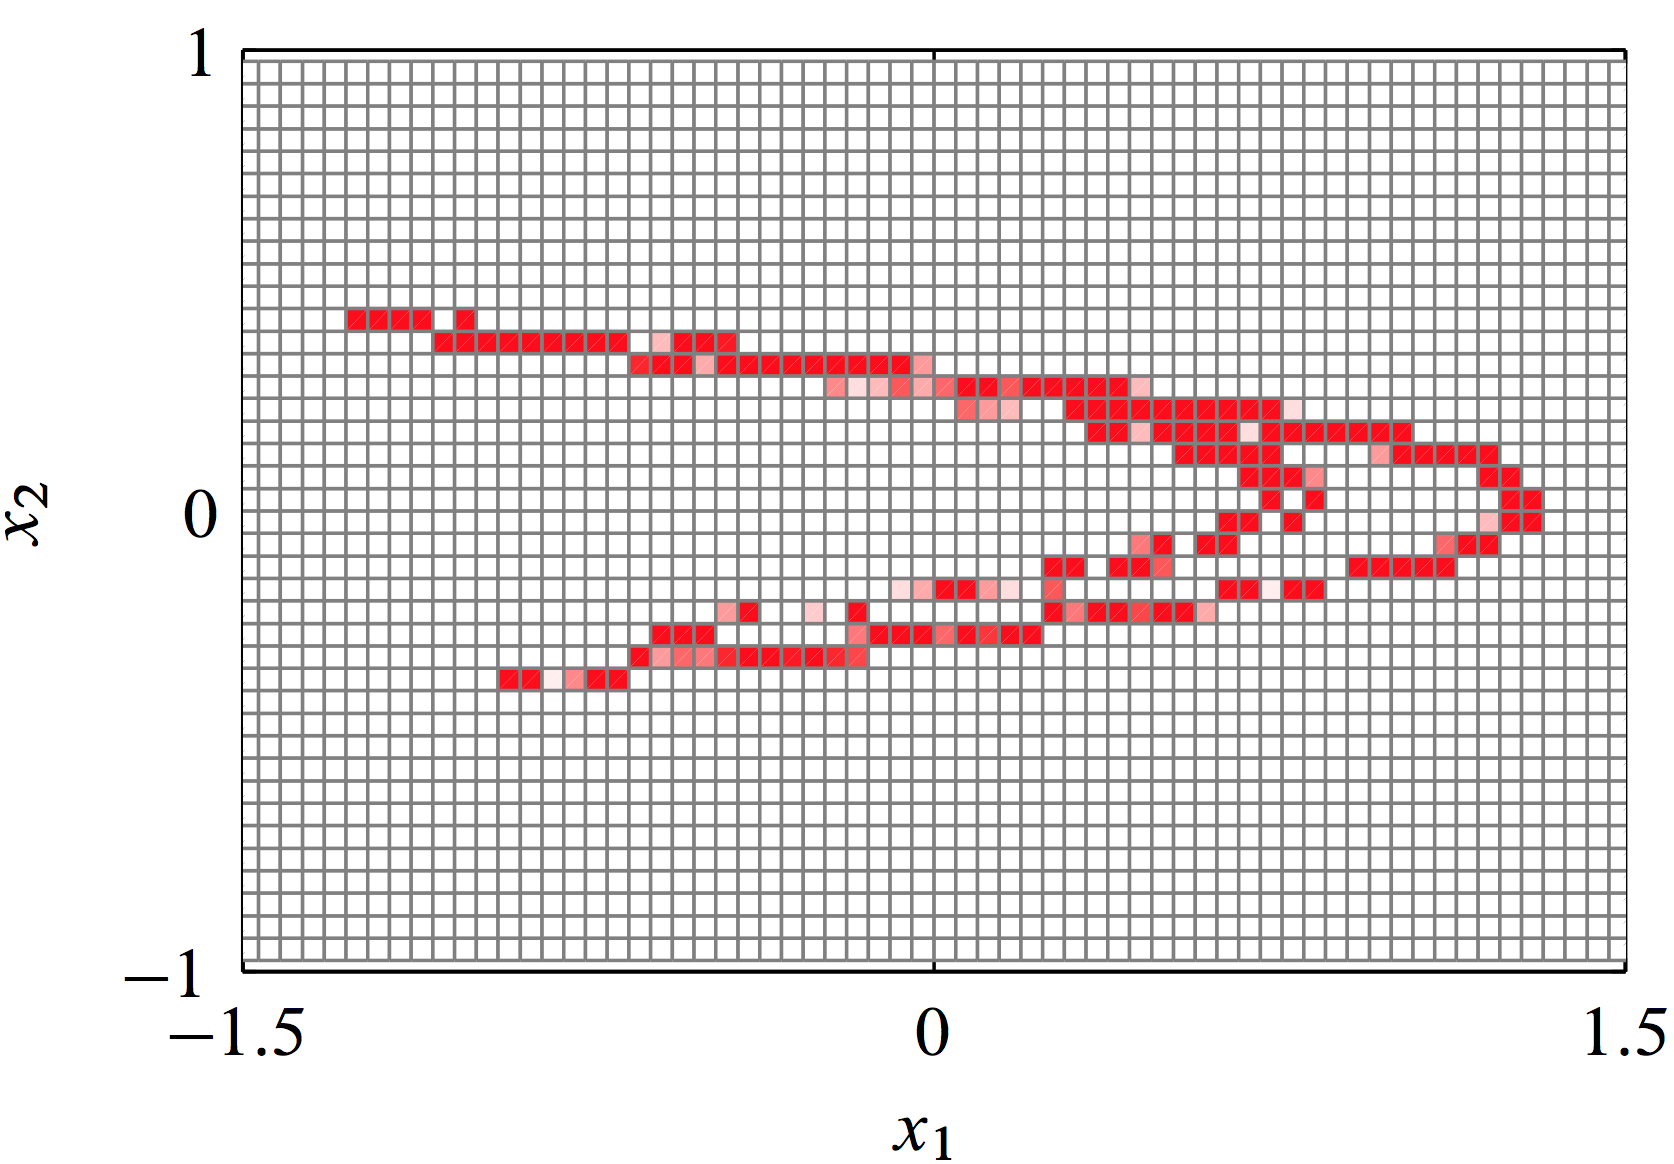
\includegraphics[width=0.35\textwidth]{henon-attr.png} }}%
    \qquad
    \subfloat{{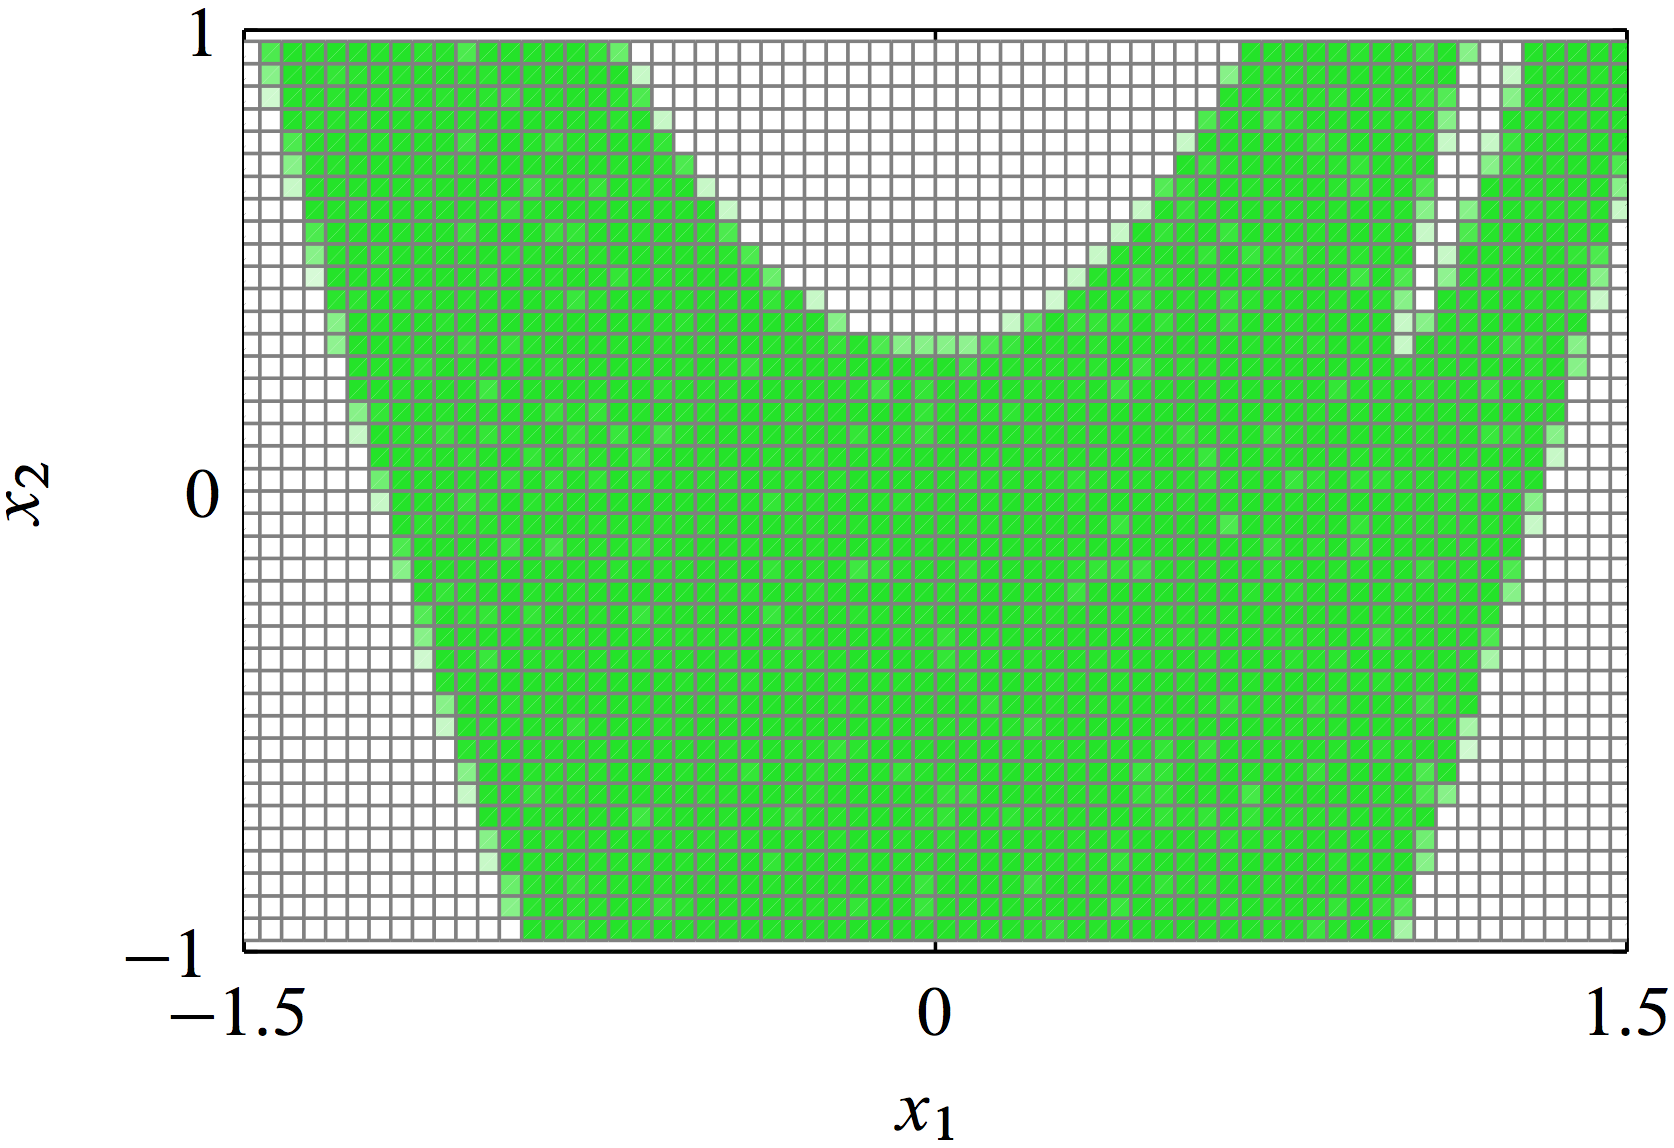
\includegraphics[width=0.35\textwidth]{henon-basin.png} }}%
\end{figure}
}

\note[itemize]{
    \item One interesting advantage of using the method is to approximate attractor and basin of attraction in a map.
    \item Let's look at the classical H\'{e}non map.. without building the transfer operator, we need around 10000 iterations of the map to identify the attractor in red and the basin of attractor i n green. 
    \item if we use a grid, perform 1 iteration of the map and build the transfer operator. Looking at the left and right eigenvector we can obtain an approximation of the attractor and its basin of attraction.
}

\frame{\frametitle{Transfer operator}
\only<1>{
\begin{itemize}
    \item Domain $X$
    \item Map $T : X \circlearrowleft$ acts on a density $f : X \to \operatorname{\mathbb R}$
\end{itemize}
}

\only<2>{ 
For all the points $\in X$, if the map $T$ is area preserving, the end result can be obtained from the Perron-Frobenius operator ($\PF$):
\begin{equation*}
  \PF f(\v x) = f \circ T^{-1}(\v x).
  \label{eq:pf_cont}
\end{equation*}
}

\only<1->{
\begin{figure}[!ht]
  \centering
  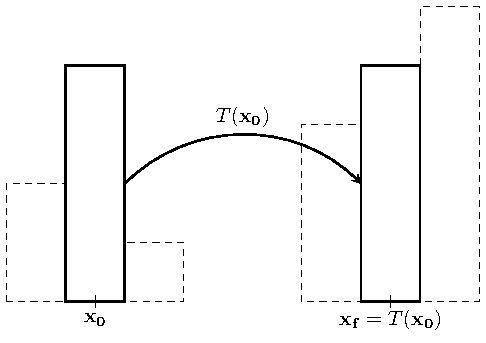
\includegraphics[scale=0.9]{fig02}
  \label{fig:push_density}
\end{figure}
}
}

\frame{\frametitle{Transition matrix \parencite{Froyland-01}}
\begin{itemize}
    \item Probabilistic approach known as Ulam's method \parencite{Ulam-79}
    \item Subdivision of the domain in boxes ($B_1, \cdots, B_n$) 
    \item From short-time trajectories, we approximate the probability to go from box $i$ to box $j$:
\end{itemize}
\begin{equation*}
\label{eq:Pij}
 \PF_{ij} \approx \frac{\#\lbrace p: p \in B_i \text{ and } T(p) \in B_j\rbrace}{\#\lbrace p \in B_i\rbrace}
\end{equation*}
by counting the number of particles (drifters) in $B_i$ that are mapped into $B_j$.
}

\note[itemize]{
    \item We are not going to exactly calculate the Perron-Frobenius operator but are going to use a probabilistic approach,  known as the Ulam's method. 
    \item The first step of the method is to subdivide the domain in boxes or bins.
    \item From short-time trajectories and for each pair of box, we approximate the probability to go from one box to the other by counting the number of particles inside the first one that are map to the second one, divided by number of particle in the first box.
}

\frame{\frametitle{Markov Chain and eigenvectors method \parencite{froyland2014well}}
\begin{itemize}
   \item $\PF$ defines a Markov Chain of the dynamics
   \item Using initial density $f_0$ $\to$ future distribution
    \begin{align}
    f_1 &= f_0 \PF\nonumber\\
    f_N &= f_0 \PF^N\nonumber
    \label{eq:pushfor}
    \end{align}
    \item left eigenvectors ($\lambda L = L \PF$)
    \begin{itemize}
        \item for $\lambda = 1$: invariant distribution
        \item for $\lambda \approx 1$: almost invariant distribution
    \end{itemize}
    \item right eigenvector highlights the basin of attraction
\end{itemize}
}

\note[itemize]{
    \item The transition matrix defines a Markov Chain of the dynamics
    \item Using this operator, and starting from a know initial density $f_0$, we can easily approximate future density distribution.
    \item Depending on their depending on their associated eigenvalues, the left eigenvectors represent an invariant distributions or some almost invariant distributions while the right eigenvectors highlight their basin of attraction. 
}

\frame{\frametitle{Example with a simple 5 states problem}

\begin{figure}[!ht]
  \centering
  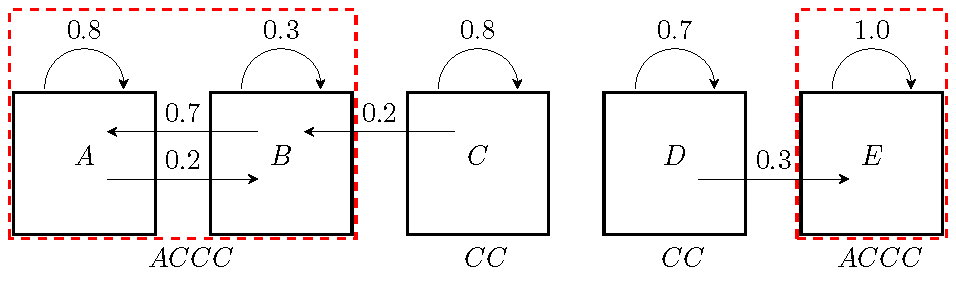
\includegraphics[width=0.9\textwidth]{fig01}
\end{figure}

\only<1>{
\begin{equation*}
\PF = 
  \begin{tabular}{c|ccccc}
    & A & B & C & D & E\\\hline
  A & 0.8 & 0.2 & 0 & 0 & 0\\
  B & 0.7 & 0.3 & 0 & 0 & 0\\
  C & 0 & 0.2 & 0.8 & 0 & 0\\
  D & 0 & 0 & 0 & 0.7 & 0.3\\
  E & 0 & 0 & 0 & 0 & 1.0
  \end{tabular}
  \label{eq:ex_pf}
\end{equation*}
}

\only<2->{
\begin{equation*}
  L_1^T = 
  \begin{pmatrix}
  0.83\\
  0.55\\
  0\\
  0\\
  0\\
  \end{pmatrix}\quad
  R_1 = 
  \begin{pmatrix}
  1\\
  1\\
  1\\
  0\\
  0\\
  \end{pmatrix}\quad
  L_2^T = 
  \begin{pmatrix}
  0\\
  0\\
  0\\
  0\\
  1\\
  \end{pmatrix}\quad
  R_2 = 
  \begin{pmatrix}
  0\\
  0\\
  0\\
  1\\
  1\\
  \end{pmatrix}
\end{equation*}

\begin{multicols}{2}
\begin{itemize}
    \item $L_1$: $A, B$ are attractors
    \item $L_2$: $E$ is another attractor
    \item $R_1$: $A, B, C$ basin of attr.
    \item $R_2$: $D, E$ basin of attr.
\end{itemize}
\end{multicols}
}
}

\section[Algorithm on real data!]{Algorithm}

\frame{\frametitle{Hypothesis}

All drifters trajectory start at the same time (Autonomous system) and we construct the transition matrix by looking where drifters end up \SI{2}{days} later (bins size, data).
   \begin{figure}
      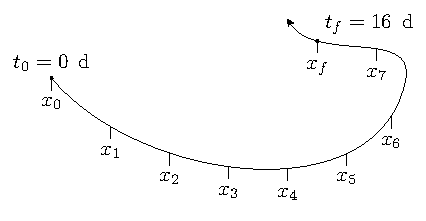
\includegraphics[width=0.7\linewidth]{fig03b}
    \end{figure}
}

\note[itemize]{
    \item But first let's remember our main hypothesis
    \item The trajectory length is selected in function of the bins size, basically we want the time to be long enough so drifters can leave the box.
    \item It is also use to increase the number of trajectories. For example, if we have a 16 d trajectory, we will split it in 8 segments that are use independently when constructing the transition matrix.
}

\frame{\frametitle{Algorithm}

\begin{enumerate}
  \item Split the domain (\gom) into square boxes
  \item For each trajectory segment:
  \begin{itemize}
    \item find bins $i$ where $x_0$ is located and store the segment $ID$ in the vector $B_i$
    \item identify bins $j$ where $x_f$ is located and store the segment $ID$ in the vector $B_j$
  \end{itemize}  
  \item Calculate the transition matrix $\PF_{ij}$ using vectors $B_i$ and $B_j$
  \item Calculate eigenvalues and eigenvectors of $\PF$
\end{enumerate}

}

\section[Let's look at the results !]{Results}


\frame{\frametitle{Strongly connected components (Tarjan algorithm)}

\textbf{The \gom\ is almost completely covered by a single CC.}

\begin{itemize}
    \item Borders: Closed Communicating Classes ($CCC$) in red with Attractive Closed Communicating Classes ($ACCC$) in black
    \item Handful of drifters and small effect on the general dynamics
\end{itemize}

\begin{figure}[!ht]
  \centering
  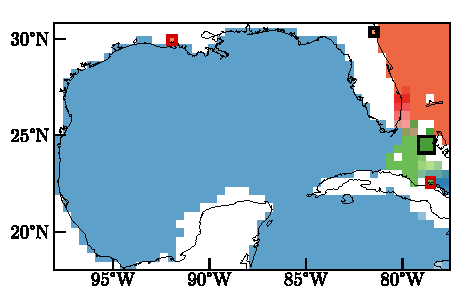
\includegraphics[width=0.8\linewidth]{fig04b}
  \label{fig:tarjan}
\end{figure}
}

\note[itemize]{
    \item On the left image, we can see that there is basically two strongly connected domain. One inside the Gulf of Mexico and the Caribbean sea while the other is in the Atlantic Ocean.
    \item on the right part we can note some Closed communicating classes that are created by drifters beaching on island in the Bahamas or on the coast of Florida.. They regroup only an handful of drifters and are not really important for the general dynamics of the \gom.
}

\frame{\frametitle{Limiting distribution from a uniform density}

\textbf{Existence of a westward mean flow}: similar to results presented by \cite{sturges2016mean} from SSH data
\begin{figure}[!ht]
  \centering
  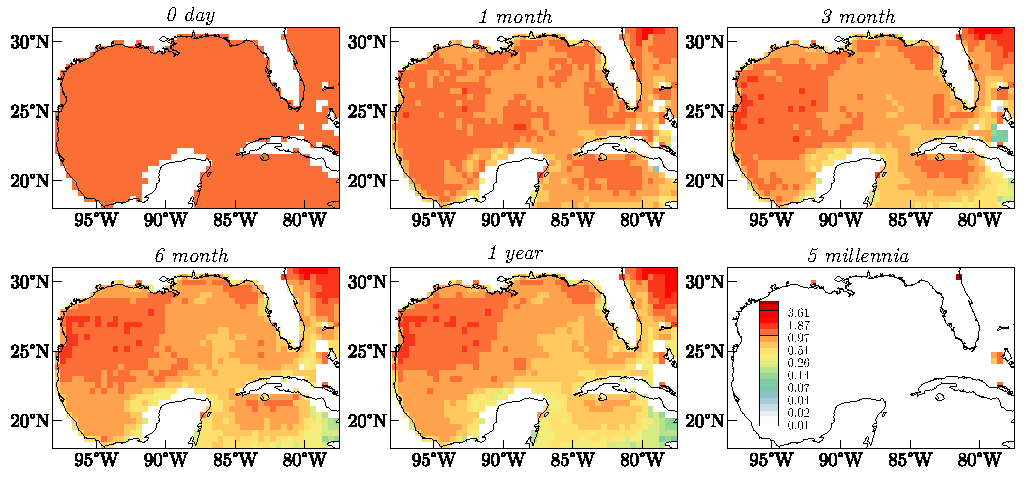
\includegraphics[width=\linewidth]{fig05b}
  \label{fig:limiting_dist}
\end{figure}
}

\note[itemize]{
    \item The limiting distribution show an accumulation of density on the west region. This highlight the existence of a westward mean flow, also presented last year by Sturges from SSH analysis.
    \item After 100 days, presented B, we can identify attractors at the South of Cuba, the West of Florida and the south west of the \gom.
    \item We can guess that they are associated with smaller eigenvalue as the density accumulate  for shorter period of time.     
}

\frame{\frametitle{Top left eigenvectors}
\begin{figure}[!ht]
  \centering
  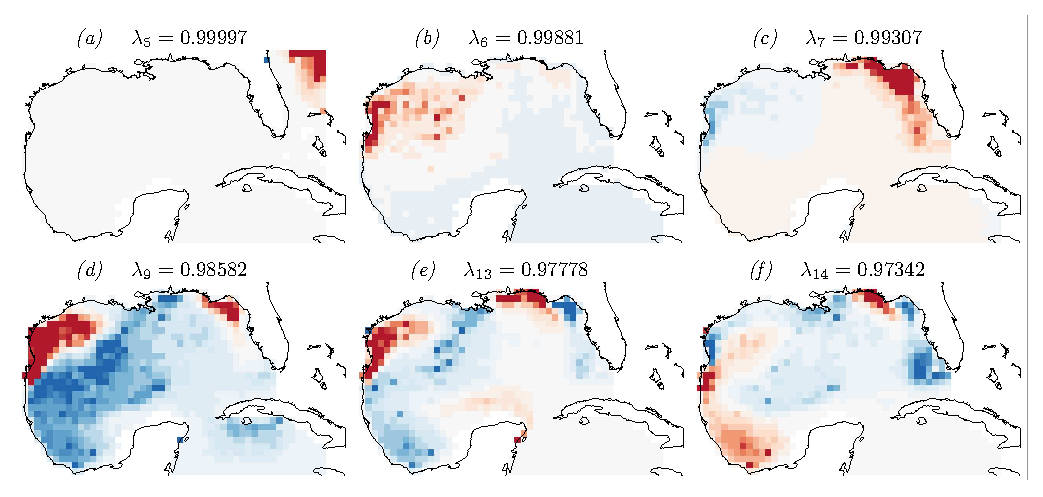
\includegraphics[width=\linewidth]{fig06}
  \label{fig:r_eig}
\end{figure}
}

\frame{\frametitle{Top right eigenvectors}

\begin{figure}[!ht]
  \centering
  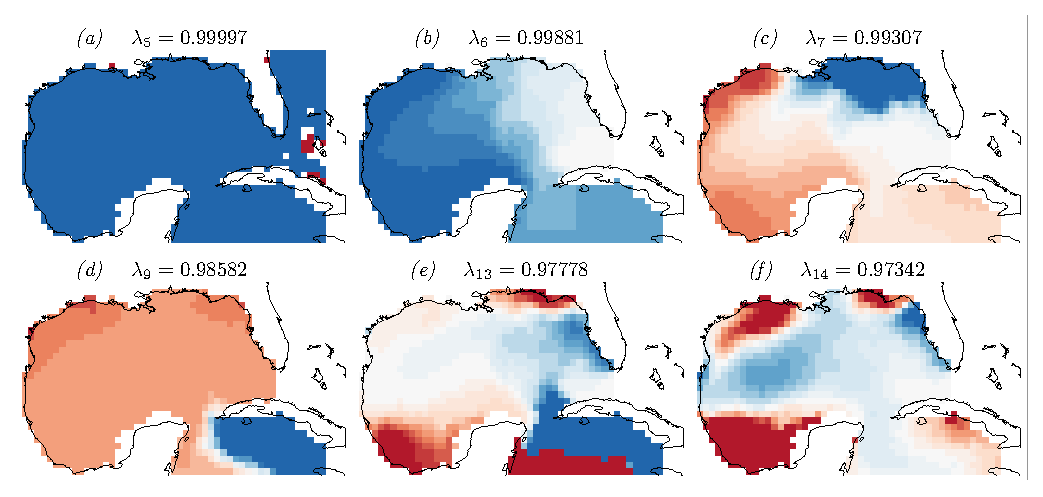
\includegraphics[width=\linewidth]{fig07}
  \label{fig:l_eig}
\end{figure}

}

\iffalse
\frame{\frametitle{Attractors converge to basins of attraction}

For the almost invariant set associated with $\lambda_6 = 0.99881$:
\begin{figure}[!ht]
  \centering
  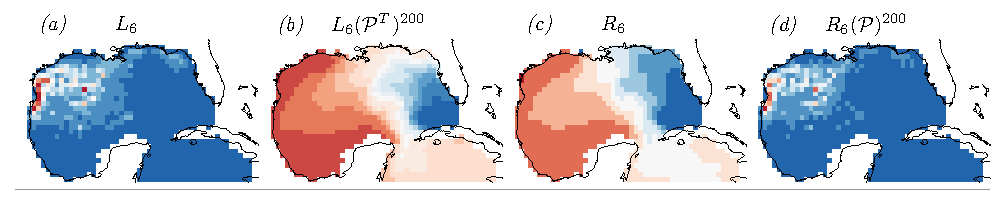
\includegraphics[width=\linewidth]{fig08}
  \label{fig:r_to_l}
\end{figure}
}
\fi

\frame{\frametitle{Dynamical geography}

\begin{itemize}
    \item \textbf{left:} the main separation of the \gom
    \item \textbf{right:} the five coastal basins of attraction
\end{itemize}

\begin{figure}[!ht]
  \centering
  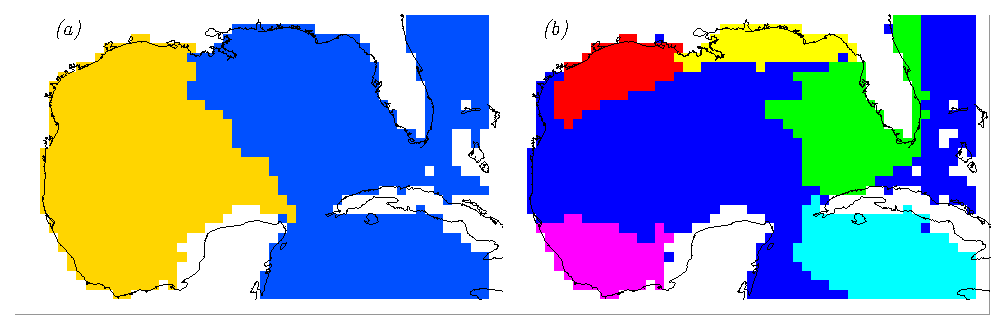
\includegraphics[width=\linewidth]{fig09}
  \label{fig:dyngeo}
\end{figure}
}

\iffalse
\frame{\frametitle{Oil rigs location}
\textbf{Distance of oil rigs from the coast is increasing in recent years..}
\begin{figure}[!ht]
  \centering
  \includegraphics[width=\linewidth]{oilrigs/fig}
  \label{fig:oilrigs}
\end{figure}
}
\fi

\section[Conclusion]{Conclusion}

\frame{\frametitle{Conclusion}
\begin{itemize}
    \item Identified \textbf{almost limiting distributions} and corresponding \textbf{basins of attraction} from the inspection of the eigenvectors
    
    \item Supported by independent observations of a westward mean flow \parencite{sturges2016mean}
    
    \item Ability to push-forward a density to "predict" the dispersion (e.g. after an oil spill or to plan a drifters experiment) 
\end{itemize}

}

\frame{\frametitle{Thank you!}
Open questions:
\begin{itemize}
    \item What is the influence of the drifters' type on the transition matrix ?
    \item Will it be possible to perform a seasonal (or maybe monthly) evaluation of the transition matrix ?
    \item How does it compare to high number of artificial drifters or simply density advection using a numerical velocity field or a global circulation model?
    \item How to "easily" extract the different sets ?
\end{itemize}
}

\frame[allowframebreaks]{\frametitle{References}
% remove References title
\begingroup
\renewcommand{\section}[2]{}%
% add cited papers
\printbibliography[heading=none]
\endgroup
}

\end{document}